\documentclass[11pt, oneside]{article}   	% use "amsart" instead of "article" for AMSLaTeX format
\usepackage{geometry}                		% See geometry.pdf to learn the layout options. There are lots.
\geometry{letterpaper}                   		% ... or a4paper or a5paper or ... 
%\geometry{landscape}                		% Activate for for rotated page geometry
%\usepackage[parfill]{parskip}    		% Activate to begin paragraphs with an empty line rather than an indent
\usepackage{graphicx}				% Use pdf, png, jpg, or eps§ with pdflatex; use eps in DVI mode
								% TeX will automatically convert eps --> pdf in pdflatex		
\usepackage{amssymb}

\title{Calibrated, Parametrized Learning}
\author{Kyle Cranmer and Daniel Whiteson}
%\date{}							% Activate to display a given date or no date

\begin{document}
\maketitle

\section{Introduction}
%\subsection{}


Notation:

\begin{itemize}
 \item $x$: a vector of observed quantities for each event (energy, momenta, angles of particles)
 \item $\theta$: parameters of a statistical model
\item $f_c(x| \theta)$:  probability density function (statistical model) for $x$ for category $c\in\{0,1\}$.
\item $s(x)$: real-valued score from a machine learning classification algorithm (or any map $s: X\to\mathbb{R}$)
\item $s(x;\theta)$: real-valued score from a parametrized machine learning classification algorithm (or any map $s: X\otimes \Theta \to\mathbb{R}$)
\item $f_c( s | \theta )$ The probability density function for $s$ implied by $f_c(x|\theta)$ and $s(x)$
\item $f_c( s(\cdot; \theta) | \theta )$ The probability density function for $s$ implied by $f_c(x|\theta)$ and $s(x;\theta)$

\end{itemize}

\subsection{Typical usage of machine learning in HEP}

In high-energy physics (HEP) we typically are searching for or measuring the properties of some 
class of events, generically referred to as \textit{signal}, in the presence of a separate class 
of \textit{background} events. For each event we measure some quantities $x$ that have corresponding distributions 
$f_0(x|\theta)$ for background and $f_1(x|\theta)$ for signal.  Often machine learning classification algorithms are trained on large samples of synthetic data $\{x_i, c_i\}$ generated with some nominal values of the parameters $\theta_0$, where $c=0$ corresponds to background and $c=1$ corresponds to signal. The resulting classifier is denoted $s(x)$. Based on this classifier and large samples of synthetic data drawn from $f_c(x | theta)$ we construct the distribution  $f_c(s | \theta)$. An example of the distributions of the distribution of $s$ for the signal and background events with $\theta=\theta_0$ is shown in Figure~\ref{fig:tmva}.


\begin{figure}[htbp]
\begin{center}
 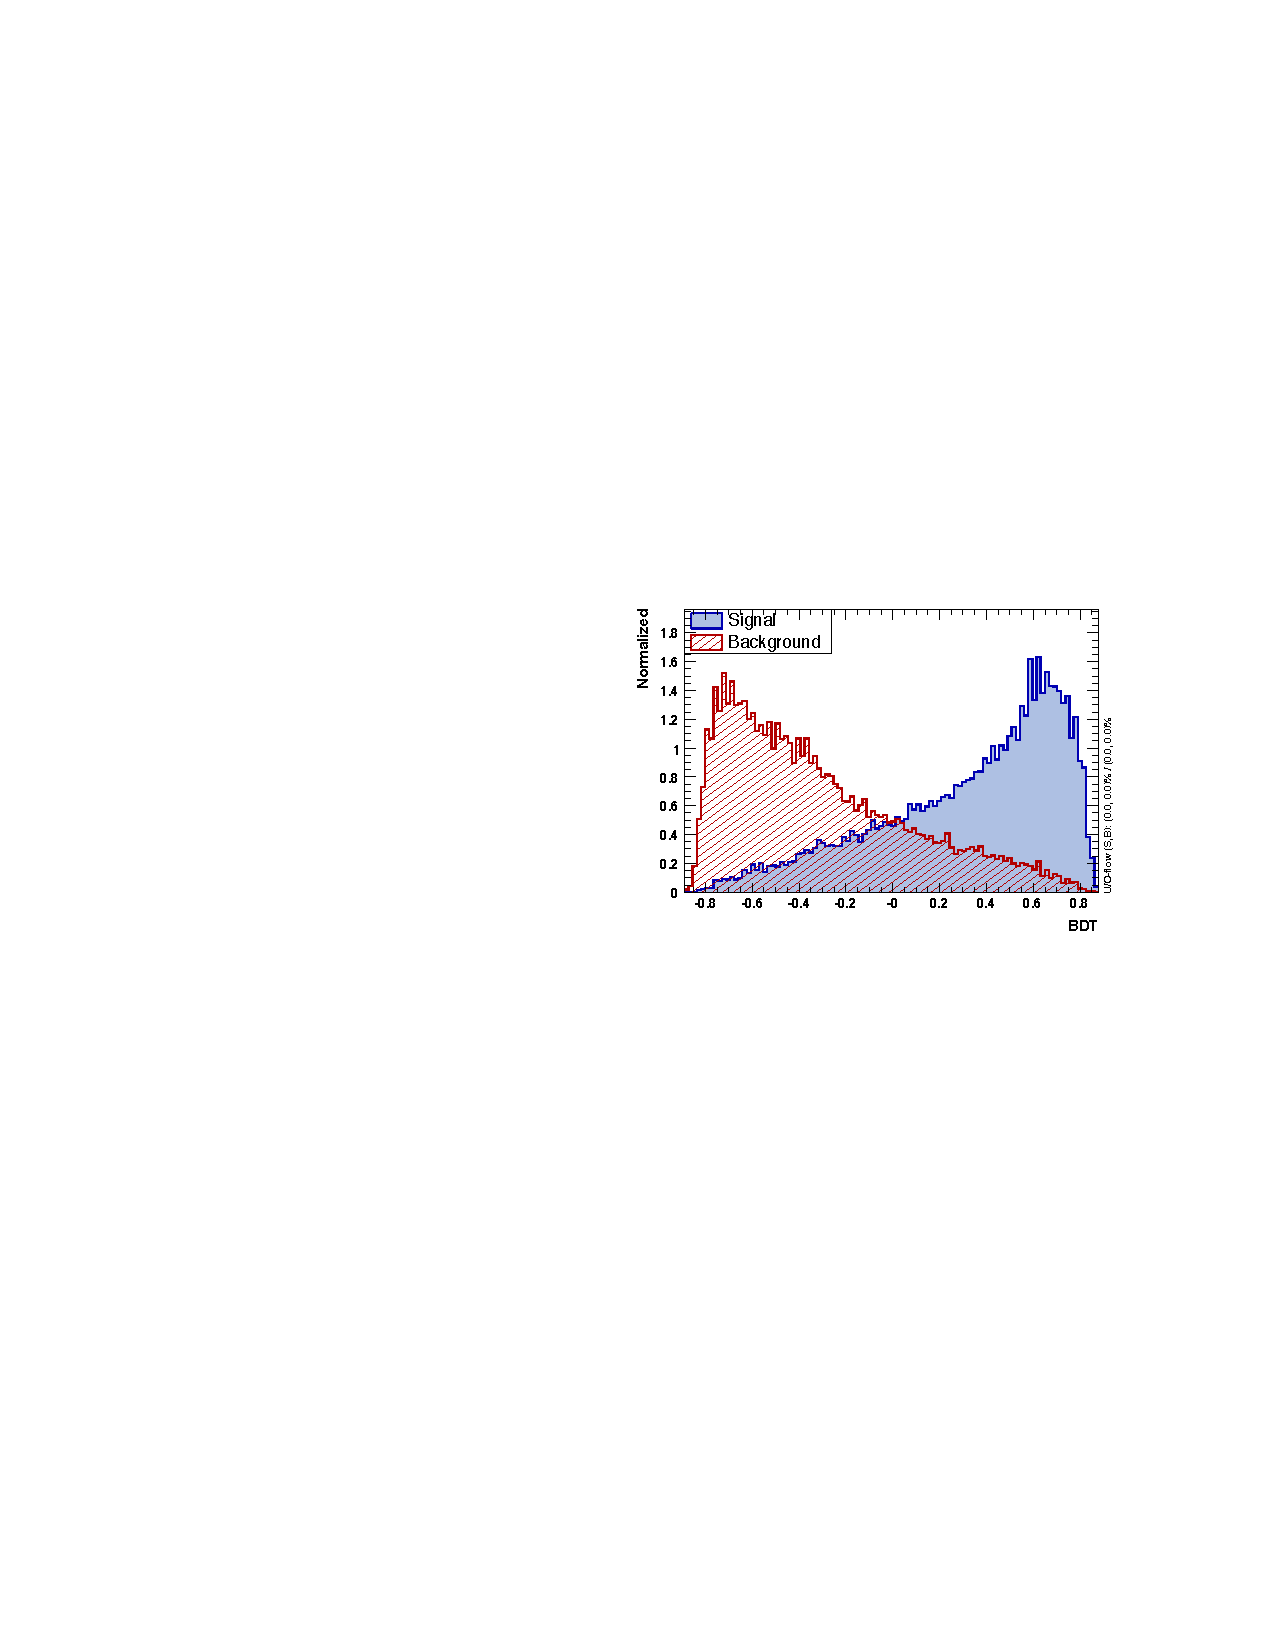
\includegraphics[height=2in]{example-TMVA-BDT.pdf}
 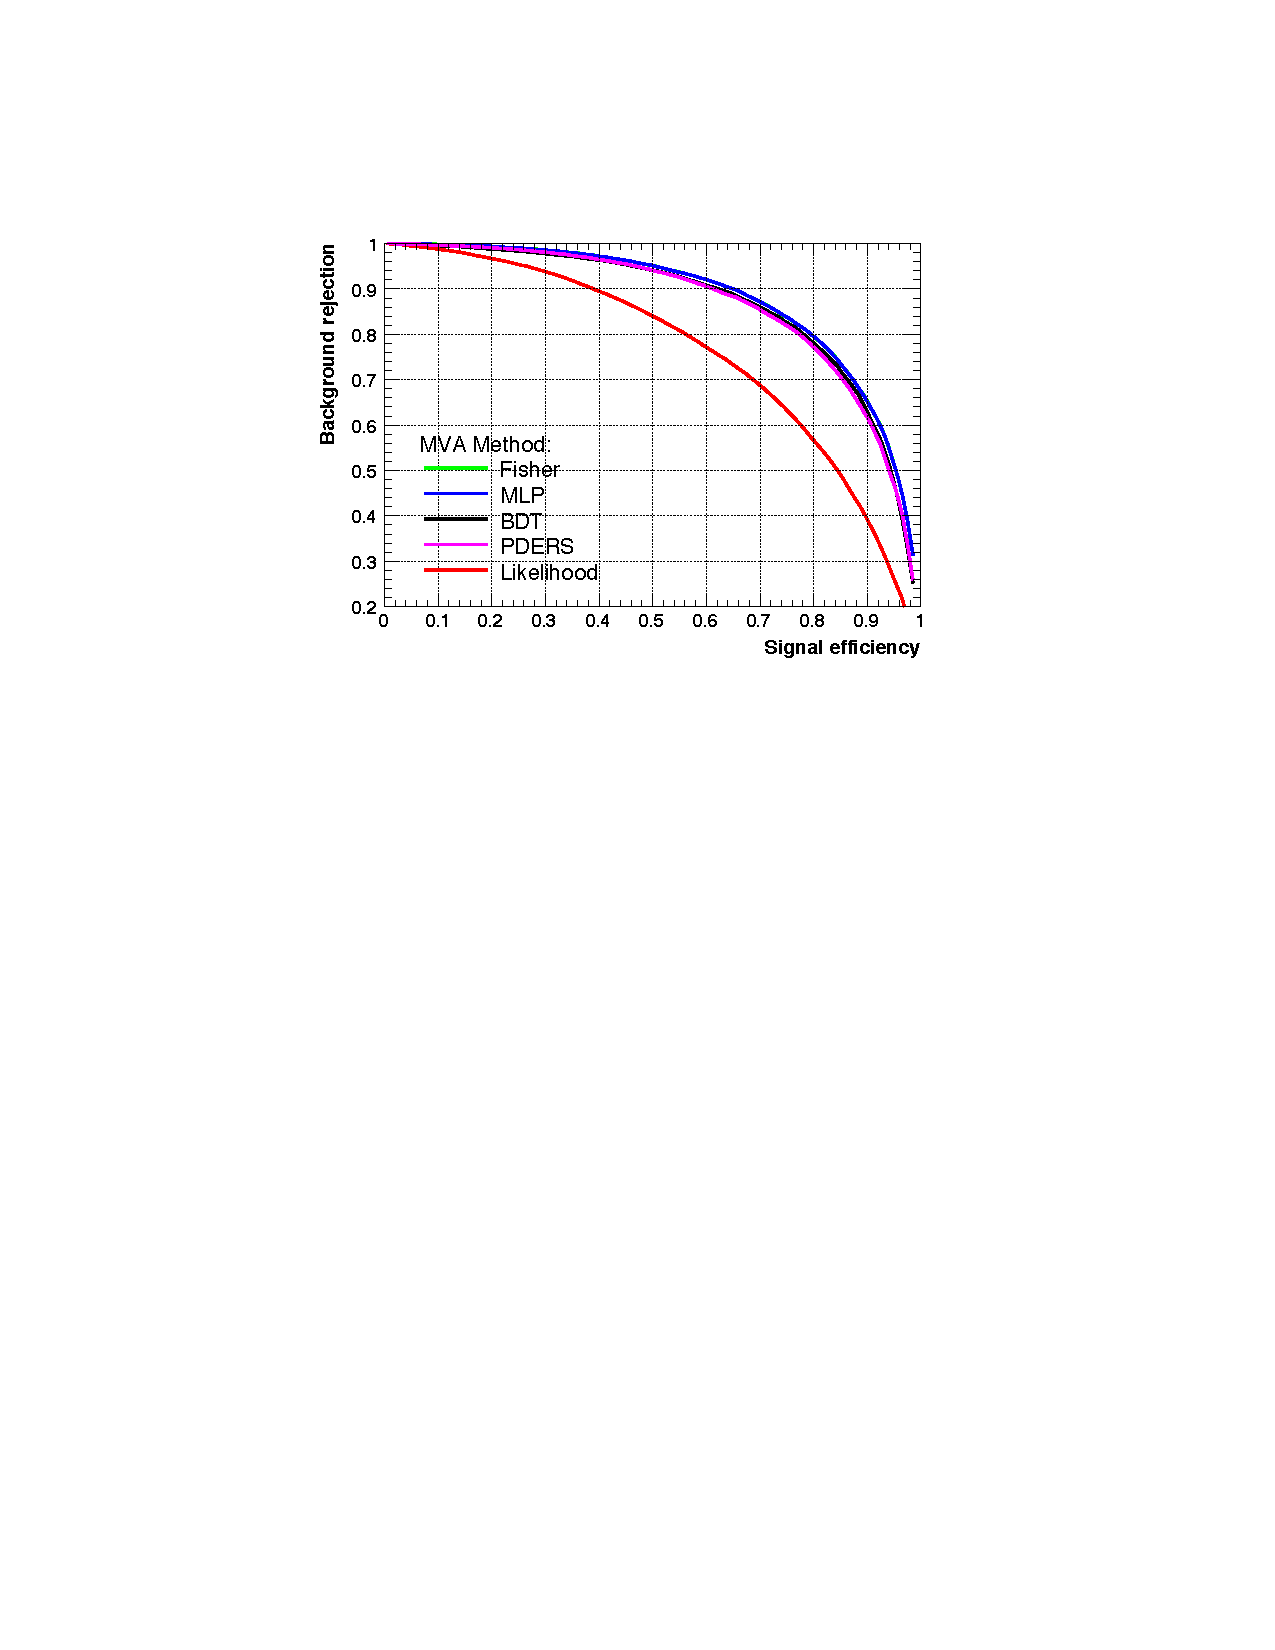
\includegraphics[height=2in]{example-TMVA-ROC.pdf}
\caption{Left: an example of the distributions $f_0(s|\theta)$ and $f_1(s|\theta)$ when the classifier $s$ is a boosted-decision tree (BDT). Right: the corresponding ROC curve (right) for this and other classifiers. Figures taken from TMVA manual.}
\label{fig:tmva}
\end{center}
\end{figure}

These steps lead to a subsequent statistical analysis where one observes in data $\{x_e\}$, where $e$ is an event index running from $1$ to $n$. For each event, the classifier is evaluated and one performs inference on a parameter $\mu$ related to the presence of the signal contribution. In particular, one forms the statistical model
\begin{equation}\label{eq:typicalML}
p( \{ x_e \} \,|\, \mu, \theta) = \prod_{e=1}^n \, \left[\, \mu f_1( s(x_e) \, |\,  \theta)  + (1-\mu)\, f_0( s(x_e) \,|\, \theta) \,\right] \; ,
\end{equation}
where $\mu=0$ is the null (background-only) hypothesis and $\mu>0$ is the alternate (signal-plus-background) hypothesis.\footnote{Sometimes there is an additional Poisson term when expected number of signal and background events is known.} Typically, we are interested in inference on $\mu$ and $\theta$ are nuisance parameters; though, sometimes $\theta$ may include some components that we are also wish to infer (like the mass of a new particle that affects the distribution $x$ for the signal events).


\subsection{Comments on typical usage of machine learning in HEP}

Nuisance parameters are an after thought in the typical usage of machine learning in HEP. In fact, most machine learning discussions would only consider $f_0(x)$ and $f_1(x)$. However, as experimentalists we know that we must account for various forms of systematic uncertainty, parametrized by $\theta$. In practice, we take the classifier as fixed and then propagate uncertainty through the classifier as in Eq.~\ref{eq:typicalML}. Building the distribution $f(s(x)|\theta)$ for values of $\theta$ other than the nominal $\theta_0$ used to train the classifier can be thought of as a calibration necessary for classical statistical inference; however, this classifier is clearly not optimal for $\theta \ne \theta_0$.

\subsection{A more powerful  approach}

The idea here is to combine the calibration of the distributions of the classifier output and a more optimal family of classifiers $s(x; \theta)$. Creating the family of classifiers is straight forward, one simply augments the training data with $x$ examples drawn from several values of $\theta$ and then includes the corresponding value of $\theta$ as an input to the classifier. Thus $\{x_e,c_e\} \to \{x_e,\theta_e, c_e\}$ leading to a parametrized learner $s(x)\to s(x;\theta)$. This leads to a complication: one does not know the value of $\theta$ to use when evaluating the parametrized classifier $s(x;\theta)$.  However, when performing statistical inference one will evaluate the likelihood of the data at a given value of $\theta$, so this is a natural choice.  Thus one arrives at the generalization of Eq.~\ref{eq:typicalML}
\begin{equation}\label{eq:parametrizedML}
p( \{ x_e \} \,|\, \mu, \theta) = \prod_{e=1}^n \, \left[\, \mu f_1( s(x_e;\theta) \, |\,  \theta)  + (1-\mu)\, f_0( s(x_e;\theta) \,|\, \theta) \,\right] \; .
\end{equation}

The construction in Eq.~\ref{eq:parametrizedML} presents a computational challenge as for each value of $\theta$ one has a new mapping $s: x\to\mathbb{R}$. The most naive realization of this would be to generate synthetic data $\{x_e\}$ according to $f_c(x|\theta)$, evaluate $s(x_e ; \theta)$, and then use a histogram, kernel density, or other non-parametric density estimation procedure to estimate $f_c( s | \theta)$. This approach is not realistic in situations where $f_c(x|\theta)$ is realized with expensive computer simulations; thus, some interpolation strategy or emulator over a fixed set of parameter points $\{\theta_i\}$ would typically be used.

\end{document} 
